\documentclass{article}
\usepackage[utf8]{inputenc}
\usepackage{graphicx}
\usepackage{listings}

\title{Algo3}
\author{Yvo Hu s2962802 }
\date{May 2021}
\maketitle
\begin{document}
\section{Introductie}
We stellen ons een belegger voor die op dag 0 een bepaald bedrag tot zijn beschikking heeft. Op
elke dag kan hij beslissen om aandelen te kopen of te verkopen. Dat gebeurt dan tegen de koersen
van de aandelen op die dag. Voor elke koop of verkoop betaalt de belegger een percentage aan
provisie. Om geen al te grote risico’s te nemen, wil de belegger niet te veel aandelen van hetzelfde
bedrijf hebben. Sterker nog: van elk bedrijf wil hij hoogstens ´e´en aandeel bezitten.
In de praktijk zal de belegger meestal ook een bedrag in kas (dus niet in aandelen) hebben. Dit
bedrag mag niet negatief worden, wat betekent dat de belegger niet altijd alles kan kopen wat
hij zou willen. Over het bedrag in kas ontvangt (of betaalt) hij rente, en die rente varieert per
dag. Na verloop van tijd wil de belegger een wereldreis gaan maken. Hij verkoopt dan al zijn
aandelen. Zijn beleggingsdoel is om bij het begin van zijn wereldreis, na verkoop van al zijn
aandelen, zo veel mogelijk geld in kas te hebben\\\\
De opdracht luidt als volgt: Bepaal het maximum bedrag dat een belegger in kas kan hebben op dag tw als hij optimale beleggingen maakt op basis van het begin bedrag, de koersen over de gehele periode, en de rentes over de gehele periode.
\section{Oplossing}
Het probleem is, bereken het maximale bedrag dat iemand in kas kan hebben op dag t $\ge$ 1 gegeven een aantal aandelen en de bijbehorende prijzen en rentes van dag 0 tot dag tw. \\\\
Hoe lossen we dit op? We berekenen iedere dag het bedrag in kas als we een bepaald aandeelbezit hebben. Dit wordt gerepresenteerd met een bitstring. De numerieke waarde van deze bitstring is maximaal $2^n - 1$ waar n staat voor het aantal aandelen waar men uit kan kiezen (255 in dit geval). \\\\Elk aandeel in de bitstring aan het begin van de dag moet worden gekocht of verkocht o.b.v. het aandeelbezit aan het einde van de vorige dag.\\\\ Op dag 0 heeft men nog geen aandelen in bezit, en berekent voor elke permutatie van de bitstring het bedrag in kas en stopt deze in een tabel. Dit kan betekenen dat het bedrag in kas in de min gaat (Deze worden overgeslagen in de berekening).
\\\\
Voor elke permutatie van de aandelenbezit bitstring waarvan het bedrag in kas $\ge$ 0 wordt tegelijkertijd berekent wat het maximale bedrag in kas is morgen als men alle aandelen in bezit verkoopt.\\\\
De beste combinatie aandelen die men moet kopen op dag t en het bijbehorende bedrag in kas die aan het einde van de dag $\ge$ 0 is + rente dienen als vervolgwaarde voor het start bedrag in kas op dag t + 1.\\\\ Misschien omgekeerd maar alle aandelen in bezit aan het eind van de vorige dag worden aan het begin van de huidige dag verkocht. De provisie voor de transactie wordt teruggestort als blijkt dat deze in de bitstring van de huidige iteratie voorkomt. Dit is dus een verkoop en een herkoop, maar we doen alsof er niets gebeurt.\\\\
Dit herhaalt zich tot dag tw. Waarna het maximale bedrag op dag tw dat men kan hebben wordt geretourneerd.\\

\newpage
Een visualisatie van de beslissingsboom\\\\
Elke dag wordt de beste combinatie van aandelen gekozen(bitstring), en het algoritme bouwt de volgende dag verder aan de hand van die beste combinatie van de vorige dag. Elke tak staat voor een bepaalde bitstring aandelenbezit. Gesnoeide takken betekenen dat er niet verder langs die tak wordt gezocht naar een 'beter' eind resultaat want dat is er niet.
\begin{figure}[htp]
    \centering
    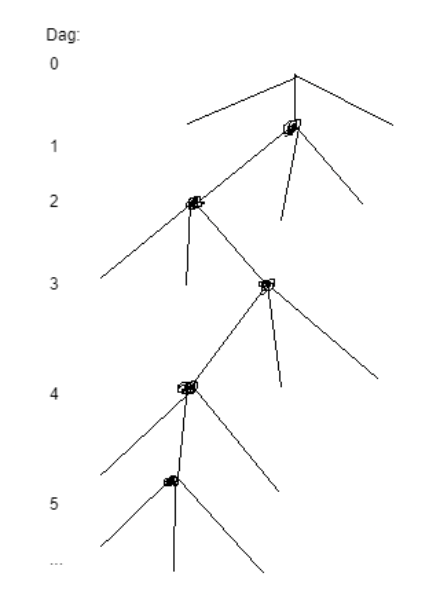
\includegraphics[width=8cm]{algo3/testtt.png}
    \label{fig:galaxy}
\end{figure}
\newpage
\subsection{Recursieve formulering}
bedrag(0,0) = beginbedrag\\
bedrag(0,a) = bedrag(0,0) - (waarde van aandelen in a * (1 + provisie)) \\\\
=====================================================\\\\
\\ \#MAXbedrag is het bedrag dat morgen in kas zit als men alle aandelen in bezit verkoopt + de rente\\\\
MAXbedrag(t+1, 0) = bedrag(t, a) waarvoor bedrag(t+1, 0) * (1 + rente(t)) is gemaximaliseert en bedrag(t,a) niet negatief is.\\
\\ \#MAXa is de bitstring a behorend bij MAXbedrag\\\\ 
=====================================================\\\\
\\ \# We beginnen de dag door elk aandeel van de vorige dag te verkopen, als blijkt dat we een aandeel willen behouden om op een latere dag te verkopen, dan storten we de transactiekosten terug in de kas.\\\\
bedrag(t, a) = MAXbedrag(t, 0)\\\\
\\ \#Verkoop van aandelen\\
+ (1 - provisie) * (waarde van aandelen in MAXa die niet in a zitten)\\
\\ \#Koop van aandelen\\
- (1 + provisie) * (waarde van aandelen in a die niet in MAXa zitten))\\
\\ \#Terugstorten van provisie \\ 
+ (provisie) * (waarde van aandelen in a die ook in MAXa zitten))
\\\\
\\\\
\newpage
\subsection{bepaalMaxBedragBU Tijdscomplexiteit}
De tijdscomplexiteit van bepaalMaxBedragBU is als volgt:\\\\
In BepaalMaxBedragBU:\\
for(int t = 0; t \textless this$\rightarrow$ tw; t++)\\
\{\\
this $\rightarrow$ berekenMaxb0(t, maxa, maxb0);\\
this $\rightarrow$ voegToeDagTransacties(maxa, transacties);\\
..
\\
\}\#O(tw)\\\\
In berekenMaxb0:\\
for(size\_t bitstring = 0; bitstring \textless dagb0.size(); bitstring++)\\
\{\\
  this$\rightarrow$vulTabel(t, dagb0)\\
  ...
\\
\}\#O(n)\\\\
In vulTabel:\\
for(int bitstring = 0; bitstring $\leq$ maxBezit; bitstring++)\\
\{\\
    for(int aandeel = 0; aandeel \textless this$\rightarrow$n; aandeel++)\\
    \{\\
    ...\\
    \}\\
..
\\
\}\#maxBezit is hier $2^{n}$ dus O($2^{n}n$) $\rightarrow$ O($2^{n}$) \\\\
In voegToeDagTransacties\\
for(int aandeel = 0; aandeel \textless this$\rightarrow$ n; aandeel++)\\
\{\\
..
\\
\}\# O(n)\\\\
Alles bij elkaar opgeteld is O(tw) + O(n) + O($2^{n}$) + O(n)\\
= O(tw) + O($2^{n}$)
\newpage
\subsection{Geheugenruimte}
Een rij voor elke dag tot tw\\
Een kolom voor elke mogelijke bitstring o.b.v. n aandelen\\
Deze tabel is dus van de vorm [tw][$2^{n}$]\\\\
We kunnen hier niet meer op bezuinigen. We moeten bijhouden wat de best mogelijke bitstring is voor een bepaalde dag. We moeten dus op z'n minst kiezen uit 1 van de$2^{n}$ mogelijkheden per dag t.
\subsection{Transacties}
We houden bij wat de transacties zijn door de best mogelijke bitstring te vergelijken met de bitstring aan het eind van de vorige dag.\\\\
Als er een aandeel mist in de nieuwe bitstring die wel in de vorige bitstring zat, dan is er sprake van een verkoop. Vice versa is er sprake van een koop. \\\\
Als een aandeel in de nieuwe bitstring overeenkomt met de vorige bitstring dan gebeurt er niets.\\\\
In drukAfTransacties is het beginbedrag gelijk aan bedrag(0,0).\\ Hier worden vervolgens alle transacties op toegepast die eerder zijn berekent. Het resultaat is het maximale eindbedrag op dag tw.
\section{Appendix}
\subsection{main}
\lstinputlisting{main.cc}
\subsection{constantes}
\lstinputlisting{constantes.h}
\subsection{standaard}
\lstinputlisting{standaard.h}
\lstinputlisting{standaard.cc}
\subsection{beurs}
\lstinputlisting{beurs.h}
\lstinputlisting{beurs.cc}
\subsection{genereerinstantie}
\lstinputlisting{genereerinstantie.cc}

\section{makefile}
\lstinputlisting{Makefile}
\lstinputlisting{MakefileGenereer}

\end{document}
